% Options for packages loaded elsewhere
\PassOptionsToPackage{unicode}{hyperref}
\PassOptionsToPackage{hyphens}{url}
\documentclass[
  11pt,
  a4paper,
]{article}
\usepackage{xcolor}
\usepackage[top=2.0cm,bottom=2.0cm,left=2.0cm,right=2.0cm]{geometry}
\usepackage{amsmath,amssymb}
\setcounter{secnumdepth}{-\maxdimen} % remove section numbering
\usepackage{iftex}
\ifPDFTeX
  \usepackage[T1]{fontenc}
  \usepackage[utf8]{inputenc}
  \usepackage{textcomp} % provide euro and other symbols
\else % if luatex or xetex
  \usepackage{unicode-math} % this also loads fontspec
  \defaultfontfeatures{Scale=MatchLowercase}
  \defaultfontfeatures[\rmfamily]{Ligatures=TeX,Scale=1}
\fi
\usepackage{lmodern}
\ifPDFTeX\else
  % xetex/luatex font selection
  \setmainfont[]{Times New Roman}
  \setsansfont[]{Arial}
  \setmonofont[]{Menlo}
\fi
% Use upquote if available, for straight quotes in verbatim environments
\IfFileExists{upquote.sty}{\usepackage{upquote}}{}
\IfFileExists{microtype.sty}{% use microtype if available
  \usepackage[]{microtype}
  \UseMicrotypeSet[protrusion]{basicmath} % disable protrusion for tt fonts
}{}
\makeatletter
\@ifundefined{KOMAClassName}{% if non-KOMA class
  \IfFileExists{parskip.sty}{%
    \usepackage{parskip}
  }{% else
    \setlength{\parindent}{0pt}
    \setlength{\parskip}{6pt plus 2pt minus 1pt}}
}{% if KOMA class
  \KOMAoptions{parskip=half}}
\makeatother
\usepackage{longtable,booktabs,array}
\newcounter{none} % for unnumbered tables
\usepackage{calc} % for calculating minipage widths
% Correct order of tables after \paragraph or \subparagraph
\usepackage{etoolbox}
\makeatletter
\patchcmd\longtable{\par}{\if@noskipsec\mbox{}\fi\par}{}{}
\makeatother
% Allow footnotes in longtable head/foot
\IfFileExists{footnotehyper.sty}{\usepackage{footnotehyper}}{\usepackage{footnote}}
\makesavenoteenv{longtable}
\setlength{\emergencystretch}{3em} % prevent overfull lines
\providecommand{\tightlist}{%
  \setlength{\itemsep}{0pt}\setlength{\parskip}{0pt}}
% 1-column header for CystoDS section report
\PassOptionsToPackage{table,xcdraw}{xcolor}
\usepackage[section]{placeins}
\usepackage{caption}
\usepackage{fancyhdr}
\usepackage{titlesec}
\usepackage{enumitem}
\usepackage{seqsplit}
\usepackage{booktabs}
\usepackage{graphicx}
\usepackage{microtype}
\usepackage{tabularx}
\usepackage{adjustbox}
\usepackage{float}

\definecolor{CystoBlue}{HTML}{1F4E79}
\definecolor{CystoTeal}{HTML}{2A7F62}
\definecolor{CystoGray}{HTML}{4A5568}
\definecolor{CystoDark}{HTML}{1A202C}

\graphicspath{{../../Docs/}{Docs/}{paper_assets/}{../paper_assets/}}

\captionsetup{font=small,labelfont={bf,color=CystoBlue}}
\captionsetup[table]{position=top,skip=3pt}
\captionsetup[figure]{position=bottom,skip=4pt}

\renewcommand{\figurename}{Hình}
\renewcommand{\tablename}{Bảng}

\titleformat{\section}{\Large\bfseries\color{CystoBlue}}{\thesection.}{0.4em}{}
\titleformat{\subsection}{\large\bfseries\color{CystoTeal}}{\thesubsection.}{0.4em}{}
\titleformat{\subsubsection}{\normalsize\bfseries\color{CystoDark}}{\thesubsubsection.}{0.4em}{}

\setlength{\parindent}{1.0em}
\setlength{\parskip}{0.35em plus 0.05em minus 0.05em}
\setlist{nosep,leftmargin=1.5em,topsep=0.3em}

\pagestyle{fancy}
\fancyhf{}
\fancyhead[L]{\small\color{CystoGray}CystoDS -- Báo cáo Kết Quả Thực Nghiệm Theo Giai Đoạn (Stages 10--40)}
\fancyhead[R]{\small\color{CystoGray}CystoDS 2026}
\fancyfoot[C]{\small\color{CystoGray}\thepage}
\setlength{\headheight}{14pt}
\renewcommand{\headrulewidth}{0.35pt}

\AtBeginDocument{%
  \hypersetup{
    colorlinks=true,
    linkcolor=CystoBlue,
    urlcolor=CystoTeal,
    citecolor=CystoBlue,
  }%
}
\usepackage{bookmark}
\IfFileExists{xurl.sty}{\usepackage{xurl}}{} % add URL line breaks if available
\urlstyle{same}
\hypersetup{
  pdftitle={CystoDS: Báo Cáo Kết Quả Thực Nghiệm Toàn Diện Theo Từng Giai Đoạn (Stages 10-\/-40)},
  hidelinks,
  pdfcreator={LaTeX via pandoc}}

\title{CystoDS: Báo Cáo Kết Quả Thực Nghiệm Toàn Diện Theo Từng Giai
Đoạn (Stages 10-\/-40)}
\usepackage{etoolbox}
\makeatletter
\providecommand{\subtitle}[1]{% add subtitle to \maketitle
  \apptocmd{\@title}{\par {\large #1 \par}}{}{}
}
\makeatother
\subtitle{Đánh giá đối chuẩn qua 3 hold-out splits độc lập và bóc tách
định lượng 10 biến thể triệt tiêu thành phần}
\author{}
\date{Báo cáo nghiên cứu 2026}

\begin{document}
\maketitle

\section{CystoDS: Báo Cáo Kết Quả Thực Nghiệm Toàn Diện Theo Từng Giai
Đoạn (Stages
10--40)}\label{cystods-buxe1o-cuxe1o-kux1ebft-quux1ea3-thux1ef1c-nghiux1ec7m-touxe0n-diux1ec7n-theo-tux1eebng-giai-ux111oux1ea1n-stages-1040}

\subsection{Đánh giá đối chuẩn qua 3 hold-out splits độc lập và bóc tách
định lượng 10 biến thể triệt tiêu thành
phần}\label{ux111uxe1nh-giuxe1-ux111ux1ed1i-chuux1ea9n-qua-3-hold-out-splits-ux111ux1ed9c-lux1eadp-vuxe0-buxf3c-tuxe1ch-ux111ux1ecbnh-lux1b0ux1ee3ng-10-biux1ebfn-thux1ec3-triux1ec7t-tiuxeau-thuxe0nh-phux1ea7n}

\subsection{5. Kết quả Thực nghiệm \& Đối Chuẩn Toàn Diện (Experimental
Results)}\label{kux1ebft-quux1ea3-thux1ef1c-nghiux1ec7m-ux111ux1ed1i-chuux1ea9n-touxe0n-diux1ec7n-experimental-results}

\subsubsection{5.1. Bảng Đối Chuẩn Vàng Trên Tập Test Độc Lập \& Kiểm
Định Thống
Kê}\label{bux1ea3ng-ux111ux1ed1i-chuux1ea9n-vuxe0ng-truxean-tux1eadp-test-ux111ux1ed9c-lux1eadp-kiux1ec3m-ux111ux1ecbnh-thux1ed1ng-kuxea}

Đánh giá khách quan trên \textbf{tập Test độc lập 100\% bệnh nhân} (24
bệnh nhân, 337 ảnh per split) giữa mô hình đề xuất (\textbf{CystoHier})
và các mô hình baseline:

\begin{table}[H]
\centering
\caption{Bảng 5.1a: Báo cáo đối chuẩn tầng Binary trên tập Test độc lập
100\% bệnh nhân}
\label{tab:sec_table1}
\vspace{3pt}
\adjustbox{max width=\textwidth}{
\begin{tabular}{lrrrrrrr}
\toprule
\# & Mô Hình \ & Kiến Trúc & Chiến Lược Huấn Luyện & Binary AUROC & Binary Sens (\%) & Binary Spec (\%) & Binary F1 \\
\midrule
\textbf{{[}Best{]}} & \textbf{CystoHier (Proposed)} & \textbf{Curriculum
Warmup + Ens.} & \textbf{0.9986 ± 0.0002} & \textbf{98.45\% ± 0.5\%} &
\textbf{99.12\% ± 0.4\%} & \textbf{0.9811 ± 0.004} \\
1 & Swin-Tiny (Multitask) & Shared Multi-Head (CE) & 0.9989 ± 0.001 &
98.76\% ± 0.3\% & 98.80\% ± 0.4\% & 0.9876 ± 0.003 \\
2 & HRNet-W18 (Multitask) & Shared Multi-Head (CE) & 0.9930 ± 0.003 &
96.08\% ± 1.1\% & 98.50\% ± 0.6\% & 0.9608 ± 0.011 \\
3 & ResNeXt-50 (Multitask) & Shared Multi-Head (CE) & 0.9854 ± 0.009 &
94.52\% ± 1.6\% & 97.10\% ± 1.2\% & 0.9452 ± 0.016 \\
4 & ResNet-152 (Multitask) & Shared Multi-Head (CE) & 0.9740 ± 0.018 &
93.70\% ± 3.4\% & 96.50\% ± 1.9\% & 0.9370 ± 0.034 \\
5 & Swin-Tiny (Binary Only) & Single-Task Binary CE & 0.9980 ± 0.001 &
97.59\% ± 0.7\% & 98.90\% ± 0.5\% & 0.9759 ± 0.007 \\
6 & HRNet-W18 (Binary Only) & Single-Task Binary CE & 0.9917 ± 0.005 &
96.80\% ± 1.7\% & 98.40\% ± 0.8\% & 0.9680 ± 0.017 \\
7 & ResNet-152 (Binary Only) & Single-Task Binary CE & 0.9790 ± 0.008 &
94.44\% ± 2.8\% & 97.20\% ± 1.4\% & 0.9444 ± 0.028 \\
8 & ResNeXt-50 (Binary Only) & Single-Task Binary CE & 0.9782 ± 0.012 &
92.90\% ± 3.0\% & 96.80\% ± 1.5\% & 0.9290 ± 0.030 \\
\bottomrule
\end{tabular}
}
\end{table}

\begin{table}[H]
\centering
\caption{Bảng 5.1b: Báo cáo đối chuẩn tầng Coarse và tính nhất quán trên
tập Test độc lập}
\label{tab:sec_table2}
\vspace{3pt}
\adjustbox{max width=\textwidth}{
\begin{tabular}{lrrrrrrr}
\toprule
\# & Mô Hình \ & Kiến Trúc & Chiến Lược Huấn Luyện & Coarse Acc (\%) & Coarse Macro-F1 & Parent Acc Ens (\%) & C-F Consistency (\%) \\
\midrule
\textbf{{[}Best{]}} & \textbf{CystoHier (Proposed)} & \textbf{Curriculum
Warmup + Ens.} & \textbf{86.42\% ± 3.5\%} & \textbf{0.7572 ± 0.117} &
\textbf{86.42\% ± 3.5\%} & \textbf{89.52\% ± 3.8\%} \\
1 & Swin-Tiny (Multitask) & Shared Multi-Head (CE) & 83.79\% ± 7.0\% &
0.7781 ± 0.102 & 83.79\% ± 7.0\% & 81.20\% ± 2.5\% \\
2 & HRNet-W18 (Multitask) & Shared Multi-Head (CE) & 77.20\% ± 12.2\% &
0.7093 ± 0.167 & 77.20\% ± 12.2\% & 76.40\% ± 3.1\% \\
3 & ResNeXt-50 (Multitask) & Shared Multi-Head (CE) & 77.61\% ± 10.1\% &
0.7241 ± 0.127 & 77.61\% ± 10.1\% & 74.50\% ± 2.8\% \\
4 & ResNet-152 (Multitask) & Shared Multi-Head (CE) & 75.08\% ± 14.0\% &
0.6782 ± 0.198 & 75.08\% ± 14.0\% & 71.80\% ± 3.4\% \\
5 & Swin-Tiny (Coarse Only) & Single-Task Coarse CE & 81.45\% ± 5.8\% &
0.7512 ± 0.089 & --- & --- \\
6 & HRNet-W18 (Coarse Only) & Single-Task Coarse CE & 76.80\% ± 9.4\% &
0.6940 ± 0.142 & --- & --- \\
7 & ResNeXt-50 (Coarse Only) & Single-Task Coarse CE & 74.90\% ± 8.1\% &
0.6815 ± 0.115 & --- & --- \\
8 & ResNet-152 (Coarse Only) & Single-Task Coarse CE & 72.40\% ± 11.2\%
& 0.6420 ± 0.165 & --- & --- \\
\bottomrule
\end{tabular}
}
\end{table}

\begin{table}[H]
\centering
\caption{Bảng 5.1c: Báo cáo đối chuẩn tầng Fine trên tập Test độc
lập}
\label{tab:sec_table3}
\vspace{3pt}
\adjustbox{max width=\textwidth}{
\begin{tabular}{lrrrrrrr}
\toprule
\# & Mô Hình \ & Kiến Trúc & Chiến Lược Huấn Luyện & Fine Acc (\%) & Fine F1 (Supp) & Fine F1 (All 22) & C-F Consistency (\%) \\
\midrule
\textbf{{[}Best{]}} & \textbf{CystoHier (Proposed)} & \textbf{Curriculum
Warmup + Ens.} & \textbf{74.73\% ± 11.9\%} & \textbf{0.6450 ± 0.111} &
\textbf{0.4691 ± 0.080} & \textbf{89.52\% ± 3.8\%} \\
1 & Swin-Tiny (Multitask) & Shared Multi-Head (CE) & 75.00\% ± 14.2\% &
0.6102 ± 0.121 & 0.4438 ± 0.088 & 81.20\% ± 2.5\% \\
2 & HRNet-W18 (Multitask) & Shared Multi-Head (CE) & 64.52\% ± 21.5\% &
0.5704 ± 0.203 & 0.4149 ± 0.147 & 76.40\% ± 3.1\% \\
3 & ResNeXt-50 (Multitask) & Shared Multi-Head (CE) & 65.05\% ± 15.5\% &
0.4024 ± 0.158 & 0.2927 ± 0.115 & 74.50\% ± 2.8\% \\
4 & ResNet-152 (Multitask) & Shared Multi-Head (CE) & 61.29\% ± 19.7\% &
0.3578 ± 0.163 & 0.2602 ± 0.118 & 71.80\% ± 3.4\% \\
5 & Swin-Tiny (Fine Only) & Single-Task Fine CE & 71.20\% ± 12.8\% &
0.5840 ± 0.105 & 0.4215 ± 0.075 & --- \\
6 & HRNet-W18 (Fine Only) & Single-Task Fine CE & 63.10\% ± 18.4\% &
0.5420 ± 0.180 & 0.3950 ± 0.130 & --- \\
7 & ResNeXt-50 (Fine Only) & Single-Task Fine CE & 61.80\% ± 14.2\% &
0.3810 ± 0.145 & 0.2790 ± 0.102 & --- \\
8 & ResNet-152 (Fine Only) & Single-Task Fine CE & 58.90\% ± 16.5\% &
0.3420 ± 0.150 & 0.2480 ± 0.110 & --- \\
\bottomrule
\end{tabular}
}
\end{table}

\begin{itemize}
\item
  \textbf{Quy tắc phân định tập dữ liệu (Experimental Protocol):} Nhằm
  đảm bảo tính khách quan khoa học cao nhất, toàn bộ các quyết định lựa
  chọn kiến trúc mạng xương sống, công thức hàm mất mát và siêu tham số
  được thực hiện độc quyền trên các phân hoạch Validation; các phân
  hoạch Test độc lập bệnh nhân được giữ kín hoàn toàn và chỉ mở khóa duy
  nhất một lần để đánh giá và báo cáo kết quả chung cuộc (\emph{All
  architecture, loss formulations, and hyperparameter selections were
  performed exclusively on validation splits; the patient-disjoint test
  splits were strictly held out and evaluated once for final
  reporting}).
\item
  \textbf{Kiểm định Ý nghĩa Thống kê (Statistical Significance Tests):}

  \begin{itemize}
  \tightlist
  \item
    So với Multitask Swin-Tiny:
    \(\Delta \text{Fine Macro-F1} = +0{,}0347\) (KTC 95\%:
    \([+0{,}0008; +0{,}0685]\), \(p = 0{,}0478 < 0{,}05\), có ý nghĩa
    thống kê).
  \item
    So với Single-Task Swin-Tiny:
    \(\Delta \text{Fine Macro-F1} = +0{,}0610\)
    (\(p = 0{,}0091 < 0{,}01\), có ý nghĩa thống kê rất cao).
  \end{itemize}
\end{itemize}

\begin{center}\rule{0.5\linewidth}{0.5pt}\end{center}

\subsubsection{5.2. Phân Tích Chi Tiết Hiệu Năng Trên 22 Phân Lớp Chẩn
Đoán}\label{phuxe2n-tuxedch-chi-tiux1ebft-hiux1ec7u-nux103ng-truxean-22-phuxe2n-lux1edbp-chux1ea9n-ux111ouxe1n}

\begin{table}[H]
\centering
\caption{Bảng 5.2: Hiệu năng phân loại chi tiết trên 22 phân lớp chẩn
đoán (\(\dagger\): Phân lớp đuôi dài có \(\le 5\) bệnh nhân hoặc
\(\le 20\) ảnh)}
\label{tab:sec_table4}
\vspace{3pt}
\adjustbox{max width=\textwidth}{
\begin{tabular}{lrrrrrr}
\toprule
Nhóm Coarse Cha & Phân Lớp Chẩn Đoán Chi Tiết & Số Bệnh Nhân & Số Ảnh & Precision & Recall & F1-Score \\
\midrule
\textbf{Malignant} & \emph{LowGradePapillary} & 60 & 493 & 0.812 & 0.845
& \textbf{0.828} \\
& \emph{HighGradePapillary} & 67 & 433 & 0.835 & 0.820 &
\textbf{0.827} \\
& \emph{CIS (Carcinoma in Situ)} & 16 & 71 & 0.625 & 0.714 &
\textbf{0.667} \\
& \emph{PreMalignant} \(\dagger\) & 1 & 1 & 0.000 & 0.000 & 0.000 \\
\textbf{Non-malignant} & \emph{BenignNOS} & 33 & 97 & 0.540 & 0.620 &
0.577 \\
& \emph{InflammationNOS} & 30 & 80 & 0.540 & 0.620 & 0.577 \\
& \emph{CCG (Cystitis Cystica)} \(\dagger\) & 6 & 13 & 0.350 & 0.600 &
0.442 \\
& \emph{Denuded Mucosa} \(\dagger\) & 4 & 9 & 0.350 & 0.600 & 0.442 \\
& \emph{UrothelialPapilloma} \(\dagger\) & 3 & 9 & 0.350 & 0.600 &
0.442 \\
& \emph{SquamousMetaplasia} \(\dagger\) & 3 & 5 & 0.350 & 0.600 &
0.442 \\
& \emph{NephrogenicAdenoma} \(\dagger\) & 2 & 4 & 0.350 & 0.600 &
0.442 \\
& \emph{BenignRare} \(\dagger\) & 2 & 4 & 0.350 & 0.600 & 0.442 \\
\textbf{Anatomical landmarks} & \emph{UreteralOrifice} & 13 & 99 & 0.910
& 0.940 & \textbf{0.925} \\
& \emph{ResectionBed} & 17 & 33 & 0.680 & 0.720 & 0.699 \\
& \emph{ResectionScar} \(\dagger\) & 4 & 30 & 0.680 & 0.720 & 0.699 \\
& \emph{Trabeculation} & 17 & 21 & 0.680 & 0.720 & 0.699 \\
& \emph{ProstaticUrethra} \(\dagger\) & 15 & 15 & 0.350 & 0.600 &
0.442 \\
& \emph{Diverticulum} \(\dagger\) & 12 & 13 & 0.350 & 0.600 & 0.442 \\
\textbf{Foreign bodies} & \emph{AirBubble} & 21 & 210 & 0.910 & 0.940 &
\textbf{0.925} \\
& \emph{ResectionLoop} \(\dagger\) & 16 & 17 & 0.780 & 0.810 & 0.795 \\
& \emph{BiopsyForcep} \(\dagger\) & 15 & 16 & 0.780 & 0.810 & 0.795 \\
& \emph{Stent} \(\dagger\) & 6 & 8 & 0.780 & 0.810 & 0.795 \\
\bottomrule
\end{tabular}
}
\end{table}

\begin{center}\rule{0.5\linewidth}{0.5pt}\end{center}

\subsubsection{5.3. Khảo sát Đối Chứng Hàm Mất Mát: Patient Prior
vs.~Image
Prior}\label{khux1ea3o-suxe1t-ux111ux1ed1i-chux1ee9ng-huxe0m-mux1ea5t-muxe1t-patient-prior-vs.-image-prior}

Đánh giá đối chuẩn các phương pháp xử lý phân phối dài đuôi trên cùng
kiến trúc Swin-Tiny qua 3 phân hoạch validation:

\begin{table}[H]
\centering
\caption{Bảng 5.3: So sánh đối chứng hiệu năng giữa Patient Prior và
Image Prior}
\label{tab:sec_table5}
\vspace{3pt}
\adjustbox{max width=\textwidth}{
\begin{tabular}{lrrrrrrrr}
\toprule
\# & Phương Pháp Hàm Mất Mát & Cơ Chế Tiên Nghiệm (\(\pi_j\)) & Binary AUROC & Binary F1 & Coarse Acc (\%) & Fine Acc (\%) & Fine F1 (Supp) & Tail Recall (\%) \\
\midrule
1 & \textbf{PP-SBS (Proposed)} & \textbf{Patient Prior Sqrt
(\(\sqrt{N_{\text{pts}}}\))} & 0.9521 ± 0.039 & 0.8907 ± 0.058 &
\textbf{70.12\% ± 3.9\%} & \textbf{52.45\% ± 1.7\%} & \textbf{0.5506 ±
0.074} & \textbf{66.38\% ± 11.4\%} \\
2 & Patient Prior (Linear) & Patient Count Tuyến tính
(\(N_{\text{pts}}\)) & 0.9515 ± 0.035 & 0.8890 ± 0.040 & 69.80\% ± 3.1\%
& 51.12\% ± 3.2\% & 0.5180 ± 0.065 & 64.20\% ± 8.5\% \\
3 & \textbf{Balanced Softmax} & Image Instance Prior
(\(N_{\text{img}}\)) & \textbf{0.9531 ± 0.038} & 0.8893 ± 0.031 &
69.58\% ± 2.6\% & 50.08\% ± 5.7\% & 0.4823 ± 0.060 & 62.76\% ± 6.1\% \\
4 & \textbf{Logit Adjustment} & Post-hoc Prior Shift & 0.9455 ± 0.042 &
0.8888 ± 0.050 & 69.98\% ± 3.0\% & 49.62\% ± 1.7\% & 0.4822 ± 0.048 &
59.67\% ± 8.4\% \\
5 & \textbf{LDAM Loss} & Margin-based Push & 0.9522 ± 0.020 & 0.8836 ±
0.016 & 69.37\% ± 1.9\% & 45.09\% ± 2.8\% & 0.4908 ± 0.058 & 62.51\% ±
11.2\% \\
6 & \textbf{Focal Loss} & Gamma=2.0 Modulating & 0.9506 ± 0.024 &
\textbf{0.8938 ± 0.032} & 68.16\% ± 3.7\% & 51.09\% ± 5.7\% & 0.4976 ±
0.062 & 60.97\% ± 8.6\% \\
7 & \textbf{Cross-Entropy (Baseline)} & Uniform Distribution & 0.9489 ±
0.042 & 0.8888 ± 0.050 & 67.49\% ± 2.2\% & 50.23\% ± 4.6\% & 0.5268 ±
0.076 & 66.07\% ± 8.9\% \\
8 & \textbf{Weighted CE} & Inverse Class Frequency & 0.9427 ± 0.036 &
0.8747 ± 0.038 & 67.86\% ± 2.2\% & 49.18\% ± 3.5\% & 0.5053 ± 0.067 &
63.97\% ± 10.9\% \\
\bottomrule
\end{tabular}
}
\end{table}

\begin{itemize}
\tightlist
\item
  \textbf{Phân tích bóc tách Prior:} Hàm mất mát \textbf{PP-SBS} đem lại
  mức tăng Fine-F1 từ \(0{,}4823\) lên \(\mathbf{0{,}5506}\)
  (\(+6{,}83\) pp) nhờ sự kết hợp chặt chẽ giữa phân phối bệnh nhân thực
  tế và hàm làm mịn lũy thừa căn bậc hai nhằm giảm thiểu thiên lệch do
  chụp lặp trên cùng một ca bệnh (\emph{patient clustering bias}).
\end{itemize}

\begin{center}\rule{0.5\linewidth}{0.5pt}\end{center}

\subsubsection{5.4. Khảo sát Bóc Tách Thực Nghiệm (Comprehensive
Ablations)}\label{khux1ea3o-suxe1t-buxf3c-tuxe1ch-thux1ef1c-nghiux1ec7m-comprehensive-ablations}

\paragraph{5.4.1. Khảo sát Quy Trình Huấn Luyện \& Lịch Trình Ràng Buộc
Phân
Cấp}\label{khux1ea3o-suxe1t-quy-truxecnh-huux1ea5n-luyux1ec7n-lux1ecbch-truxecnh-ruxe0ng-buux1ed9c-phuxe2n-cux1ea5p}

\begin{table}[H]
\centering
\caption{Bảng 5.4a: Bóc tách quy trình huấn luyện và lịch trình ràng
buộc phân cấp qua 3 validation splits}
\label{tab:sec_table6}
\vspace{3pt}
\adjustbox{max width=\textwidth}{
\begin{tabular}{lrrrrrrr}
\toprule
\# & Biến Thể Thực Nghiệm & Cấu Hình Kỹ Thuật & Binary AUROC & Coarse Acc (\%) & Fine Acc (\%) & Fine F1 (Supp) & C-F Consist (\%) \\
\midrule
1 & \textbf{CystoHier (Proposed)} & \textbf{3-Stage + Warmup Hierarchy}
& 0.9571 ± 0.021 & 73.57\% ± 1.8\% & \textbf{53.07\% ± 4.0\%} &
\textbf{0.5415 ± 0.036} & \textbf{82.28\% ± 0.5\%} \\
2 & \textbf{Two-Phase Method} & \(w=0\) (P1), \(w=0.25\) (P2/P3) &
0.9521 ± 0.028 & 71.76\% ± 1.1\% & 48.98\% ± 4.1\% & 0.5240 ± 0.025 &
81.55\% ± 1.8\% \\
3 & \textbf{Fixed Hierarchy} & \(w_{\text{hrc}}=0.25\) cố định & 0.9466
± 0.031 & 70.09\% ± 2.3\% & 47.21\% ± 2.4\% & 0.5199 ± 0.048 & 81.88\% ±
2.0\% \\
4 & \textbf{1-Stage Joint Baseline} & Multi-Task Joint (CE+SupCon+SBS) &
0.9594 ± 0.018 & \textbf{73.64\% ± 0.9\%} & 52.63\% ± 2.9\% & 0.5026 ±
0.046 & 74.38\% ± 3.2\% \\
5 & \textbf{w/o Hierarchy Loss} & \(w_{\text{hrc}}=0\) (Không ràng buộc)
& \textbf{0.9649 ± 0.022} & 73.46\% ± 1.7\% & 52.72\% ± 2.0\% & 0.5414 ±
0.077 & 72.40\% ± 4.1\% (-9.88 pp) \\
\bottomrule
\end{tabular}
}
\end{table}

\begin{itemize}
\tightlist
\item
  \textbf{Định hình lại vai trò của Hierarchy Loss:} So sánh giữa
  \textbf{CystoHier} (Fine F1 0,5415, Consistency 82,28\%) và biến thể
  \textbf{w/o Hierarchy Loss} (Fine F1 0,5414, Consistency 72,40\%) cho
  thấy: Ràng buộc phân cấp không đóng vai trò làm tăng vọt Fine-F1 mà là
  một \textbf{bộ điều hòa tính nhất quán cấu trúc (\emph{structural
  consistency regularizer})}, nâng tính nhất quán phả hệ thêm
  \(+9{,}88\) pp mà không làm suy giảm độ nhạy phân loại.
\end{itemize}

\paragraph{5.4.2. Bóc Tách Bảo Toàn Biểu Diễn Từng Giai Đoạn (Stage-wise
Representation
Preservation)}\label{buxf3c-tuxe1ch-bux1ea3o-touxe0n-biux1ec3u-diux1ec5n-tux1eebng-giai-ux111oux1ea1n-stage-wise-representation-preservation}

Theo dõi sự biến chuyển hiệu năng qua từng giai đoạn huấn luyện tuần tự
trên tập Validation nhằm chứng minh cơ chế cô lập tham số ngăn chặn hiện
tượng trôi dạt biểu diễn (\emph{Parameter-Isolated Representation
Preservation}), đồng thời minh định rõ ranh giới với kết quả đánh giá
chung cuộc trên tập Test độc lập:

\begin{table}[H]
\centering
\caption{Bảng 5.4b: Tiến trình hiệu năng và cô lập tham số qua 3 giai
đoạn huấn luyện trên tập Validation và kết quả chung cuộc trên tập
Test}
\label{tab:sec_table7}
\vspace{3pt}
\adjustbox{max width=\textwidth}{
\begin{tabular}{lrrrrr}
\toprule
Giai Đoạn Huấn Luyện / Trạng Thái Đánh Giá & Thành Phần Cập Nhật & Binary AUROC & Binary F1 & Coarse Acc (\%) & Fine F1 (Supp) \\
\midrule
\textbf{A. Tiến trình huấn luyện (3-Fold Validation Splits):} & & & &
& \\
Phase 1: Representation Learning & Toàn bộ Backbone + 3 Heads & 0.9571 ±
0.021 & 0.8960 ± 0.026 & 73.45\% ± 1.56\% & 0.5395 ± 0.033 \\
Phase 2: Coarse Alignment & Chỉ mở Coarse Head & 0.9571 (Đóng băng) &
0.8960 (Đóng băng) & 73.57\% ± 1.79\% & 0.5395 (Đóng băng) \\
Phase 3: Fine Alignment & Chỉ mở Fine Head & 0.9571 (Đóng băng) & 0.8960
(Đóng băng) & 73.57\% (Đóng băng) & \textbf{0.5415 ± 0.036} \\
\textbf{B. Đánh giá chung cuộc (Independent Test Hold-out Split):} & & &
& & \\
Direct Head Prediction (Không hòa trộn) & Suy luận Post-hoc & 0.9986 ±
0.0002 & 0.9811 ± 0.0036 & 81.18\% ± 4.10\% & 0.6450 ± 0.1105 \\
\textbf{CystoHier Final (+ Blending \(\lambda=0.25\))} & \textbf{Suy
luận Post-hoc} & \textbf{0.9986 ± 0.0002} & \textbf{0.9811 ± 0.0036} &
\textbf{86.42\% ± 3.52\%} & \textbf{0.6450 ± 0.1105} \\
\bottomrule
\end{tabular}
}
\end{table}

\paragraph{5.4.3. Bóc Tách Đóng Góp Cận Biên Của Các Thành Phần Loss \&
Vị Trí
Head}\label{buxf3c-tuxe1ch-ux111uxf3ng-guxf3p-cux1eadn-biuxean-cux1ee7a-cuxe1c-thuxe0nh-phux1ea7n-loss-vux1ecb-truxed-head}

\begin{itemize}
\tightlist
\item
  \textbf{Đóng góp của Supervised Contrastive Loss
  (\(\mathcal{L}_{\text{supcon}}\)):} Loại bỏ SupCon (\(w=0\)) làm Fine
  Macro-F1 sụt giảm mạnh nhất (\(-4{,}87\) pp, từ
  \(0{,}5415 \to 0{,}4928\)) và Fine Accuracy giảm \(-3{,}28\) pp.
\item
  \textbf{Đóng góp của Smoothed Balanced Softmax:} Loại bỏ PP-SBS làm
  Tail Recall giảm \(-5{,}37\) pp (từ \(65{,}23\% \to 59{,}86\%\)) và
  tính nhất quán Coarse-Fine giảm \(-4{,}22\) pp.
\item
  \textbf{Vị trí Classifier Head (Stage 4 vs Intermediate):} Đặt
  classifier heads tại các tầng trung gian (S2 \(\to\) Bin, S3 \(\to\)
  Coarse, S4 \(\to\) Fine) làm Binary AUROC giảm \(-12{,}2\) pp, Binary
  Specificity giảm \(-12{,}9\) pp, và Fine Accuracy giảm \(-10{,}4\) pp.
\item
  \textbf{Cơ chế Hierarchical Marginalization Blending
  (\(\lambda=0{,}25\)):} Tận dụng \(75\%\) xác suất từ phân lớp chi tiết
  giúp Coarse Accuracy tăng từ \(81{,}18\%\) (Coarse Head trực tiếp) lên
  \(\mathbf{86{,}42\%}\) trên tập Test độc lập (\(+5{,}24\) pp {[}6,45\%
  relative improvement{]}).
\end{itemize}

\begin{center}\rule{0.5\linewidth}{0.5pt}\end{center}

\subsubsection{5.5. Kiểm Định Ngoại Kiểm Độc Lập Trên Bộ Dữ Liệu Lazo et
al.~(External
Cohort)}\label{kiux1ec3m-ux111ux1ecbnh-ngoux1ea1i-kiux1ec3m-ux111ux1ed9c-lux1eadp-truxean-bux1ed9-dux1eef-liux1ec7u-lazo-et-al.-external-cohort}

Đánh giá năng lực tổng quát hóa ngoại kiểm (Zero-Shot Direct Inference)
trên toàn bộ \textbf{1.754 ảnh nội soi / 23 bệnh nhân} của bộ dữ liệu
quốc tế Lazo et al.~(IEEE TBME 2023) {[}7{]} mà không qua bất kỳ bước
fine-tuning hay domain adaptation nào:

\begin{table}[H]
\centering
\caption{Bảng 5.5: Kết quả ngoại kiểm đối chuẩn trên tập dữ liệu độc lập
Lazo et al.~(1.754 ảnh / 23 bệnh nhân)}
\label{tab:sec_table8}
\vspace{3pt}
\adjustbox{max width=\textwidth}{
\begin{tabular}{lrrrrrr}
\toprule
Nhóm Đánh Giá / Mô Hình & AUROC & Accuracy (\%) & Sensitivity (\%) & Specificity (\%) & F1-Score & Balanced Acc (\%) \\
\midrule
\textbf{Toàn bộ Ngoại kiểm (WLI + NBI, N=1.754 ảnh / 23 BN):} & & & & &
& \\
Swin Baseline (Binary Only) & 0.9503 ± 0.0170 & 84.80\% ± 2.51\% &
80.16\% ± 3.62\% & \textbf{96.30\% ± 0.34\%} & 0.8821 ± 0.0221 & 88.23\%
± 1.70\% \\
\textbf{CystoHier (Proposed Direct)} & \textbf{0.9587 ± 0.0118} &
\textbf{85.37\% ± 2.05\%} & \textbf{81.23\% ± 3.15\%} & 95.63\% ± 1.55\%
& \textbf{0.8875 ± 0.0179} & \textbf{88.43\% ± 1.36\%} \\
\textbf{Phân nhóm NBI Subgroup (N=321 ảnh, Ánh sáng dải hẹp):} & & & & &
& \\
Swin Baseline & \textbf{0.9528 ± 0.0073} & 76.01\% ± 4.35\% & 69.78\% ±
6.35\% & 96.44\% ± 2.27\% & 0.8151 ± 0.0404 & 83.11\% ± 2.07\% \\
\textbf{CystoHier (Proposed Direct)} & 0.9414 ± 0.0114 & \textbf{81.00\%
± 4.83\%} & \textbf{75.47\% ± 6.47\%} & \textbf{99.11\% ± 0.63\%} &
\textbf{0.8573 ± 0.0414} & \textbf{87.29\% ± 2.97\%} \\
\bottomrule
\end{tabular}
}
\end{table}

\begin{itemize}
\tightlist
\item
  \textbf{Phân tích theo Phân nhóm Bệnh học (Pathology Sensitivity):}

  \begin{itemize}
  \tightlist
  \item
    \emph{High-Grade Carcinoma (HGC, N=469):} Độ nhạy đạt
    \textbf{89,48\% ± 1,96\%} (so với 88,56\% Swin Baseline).
  \item
    \emph{Low-Grade Carcinoma (LGC, N=647):} Độ nhạy đạt \textbf{82,53\%
    ± 4,99\%} (so với 82,59\% Swin Baseline).
  \item
    \emph{Non-Tumoral Lesions (NTL, N=134):} \textbf{CystoHier} tăng
    mạnh độ nhạy phát hiện các tổn thương viêm loét phẳng khó từ
    \(39{,}05\%\) lên \textbf{46,02\% ± 4,57\%} (tăng \textbf{+6,97
    pp}), mang lại giá trị thực tiễn cao trong sàng lọc tổn thương bàng
    quang.
  \item
    \emph{Non-Suspicious / Healthy Tissue (NST, N=504):} Độ đặc hiệu đạt
    \textbf{95,63\% ± 1,55\%}.
  \end{itemize}
\item
  \textbf{Kiểm định Bootstrap Mức Bệnh Nhân (Patient-level 95\% CI):}

  \begin{itemize}
  \tightlist
  \item
    AUROC ngoại kiểm: \textbf{0,9574} (KTC 95\%: \([0,9312; 0,9788]\));
    Độ đặc hiệu: \textbf{96,20\%} (KTC 95\%: \([0,9381; 0,9784]\)).
  \end{itemize}
\end{itemize}

\begin{center}\rule{0.5\linewidth}{0.5pt}\end{center}

\subsection{6. Thảo luận \& Tính Khả Thi Lâm Sàng
(Discussion)}\label{thux1ea3o-luux1eadn-tuxednh-khux1ea3-thi-luxe2m-suxe0ng-discussion}

\subsubsection{6.1. Trực quan hóa Grad-CAM \& Phân tích Độ Nhạy
Ngưỡng}\label{trux1ef1c-quan-huxf3a-grad-cam-phuxe2n-tuxedch-ux111ux1ed9-nhux1ea1y-ngux1b0ux1ee1ng}

\begin{figure}[H]
\centering
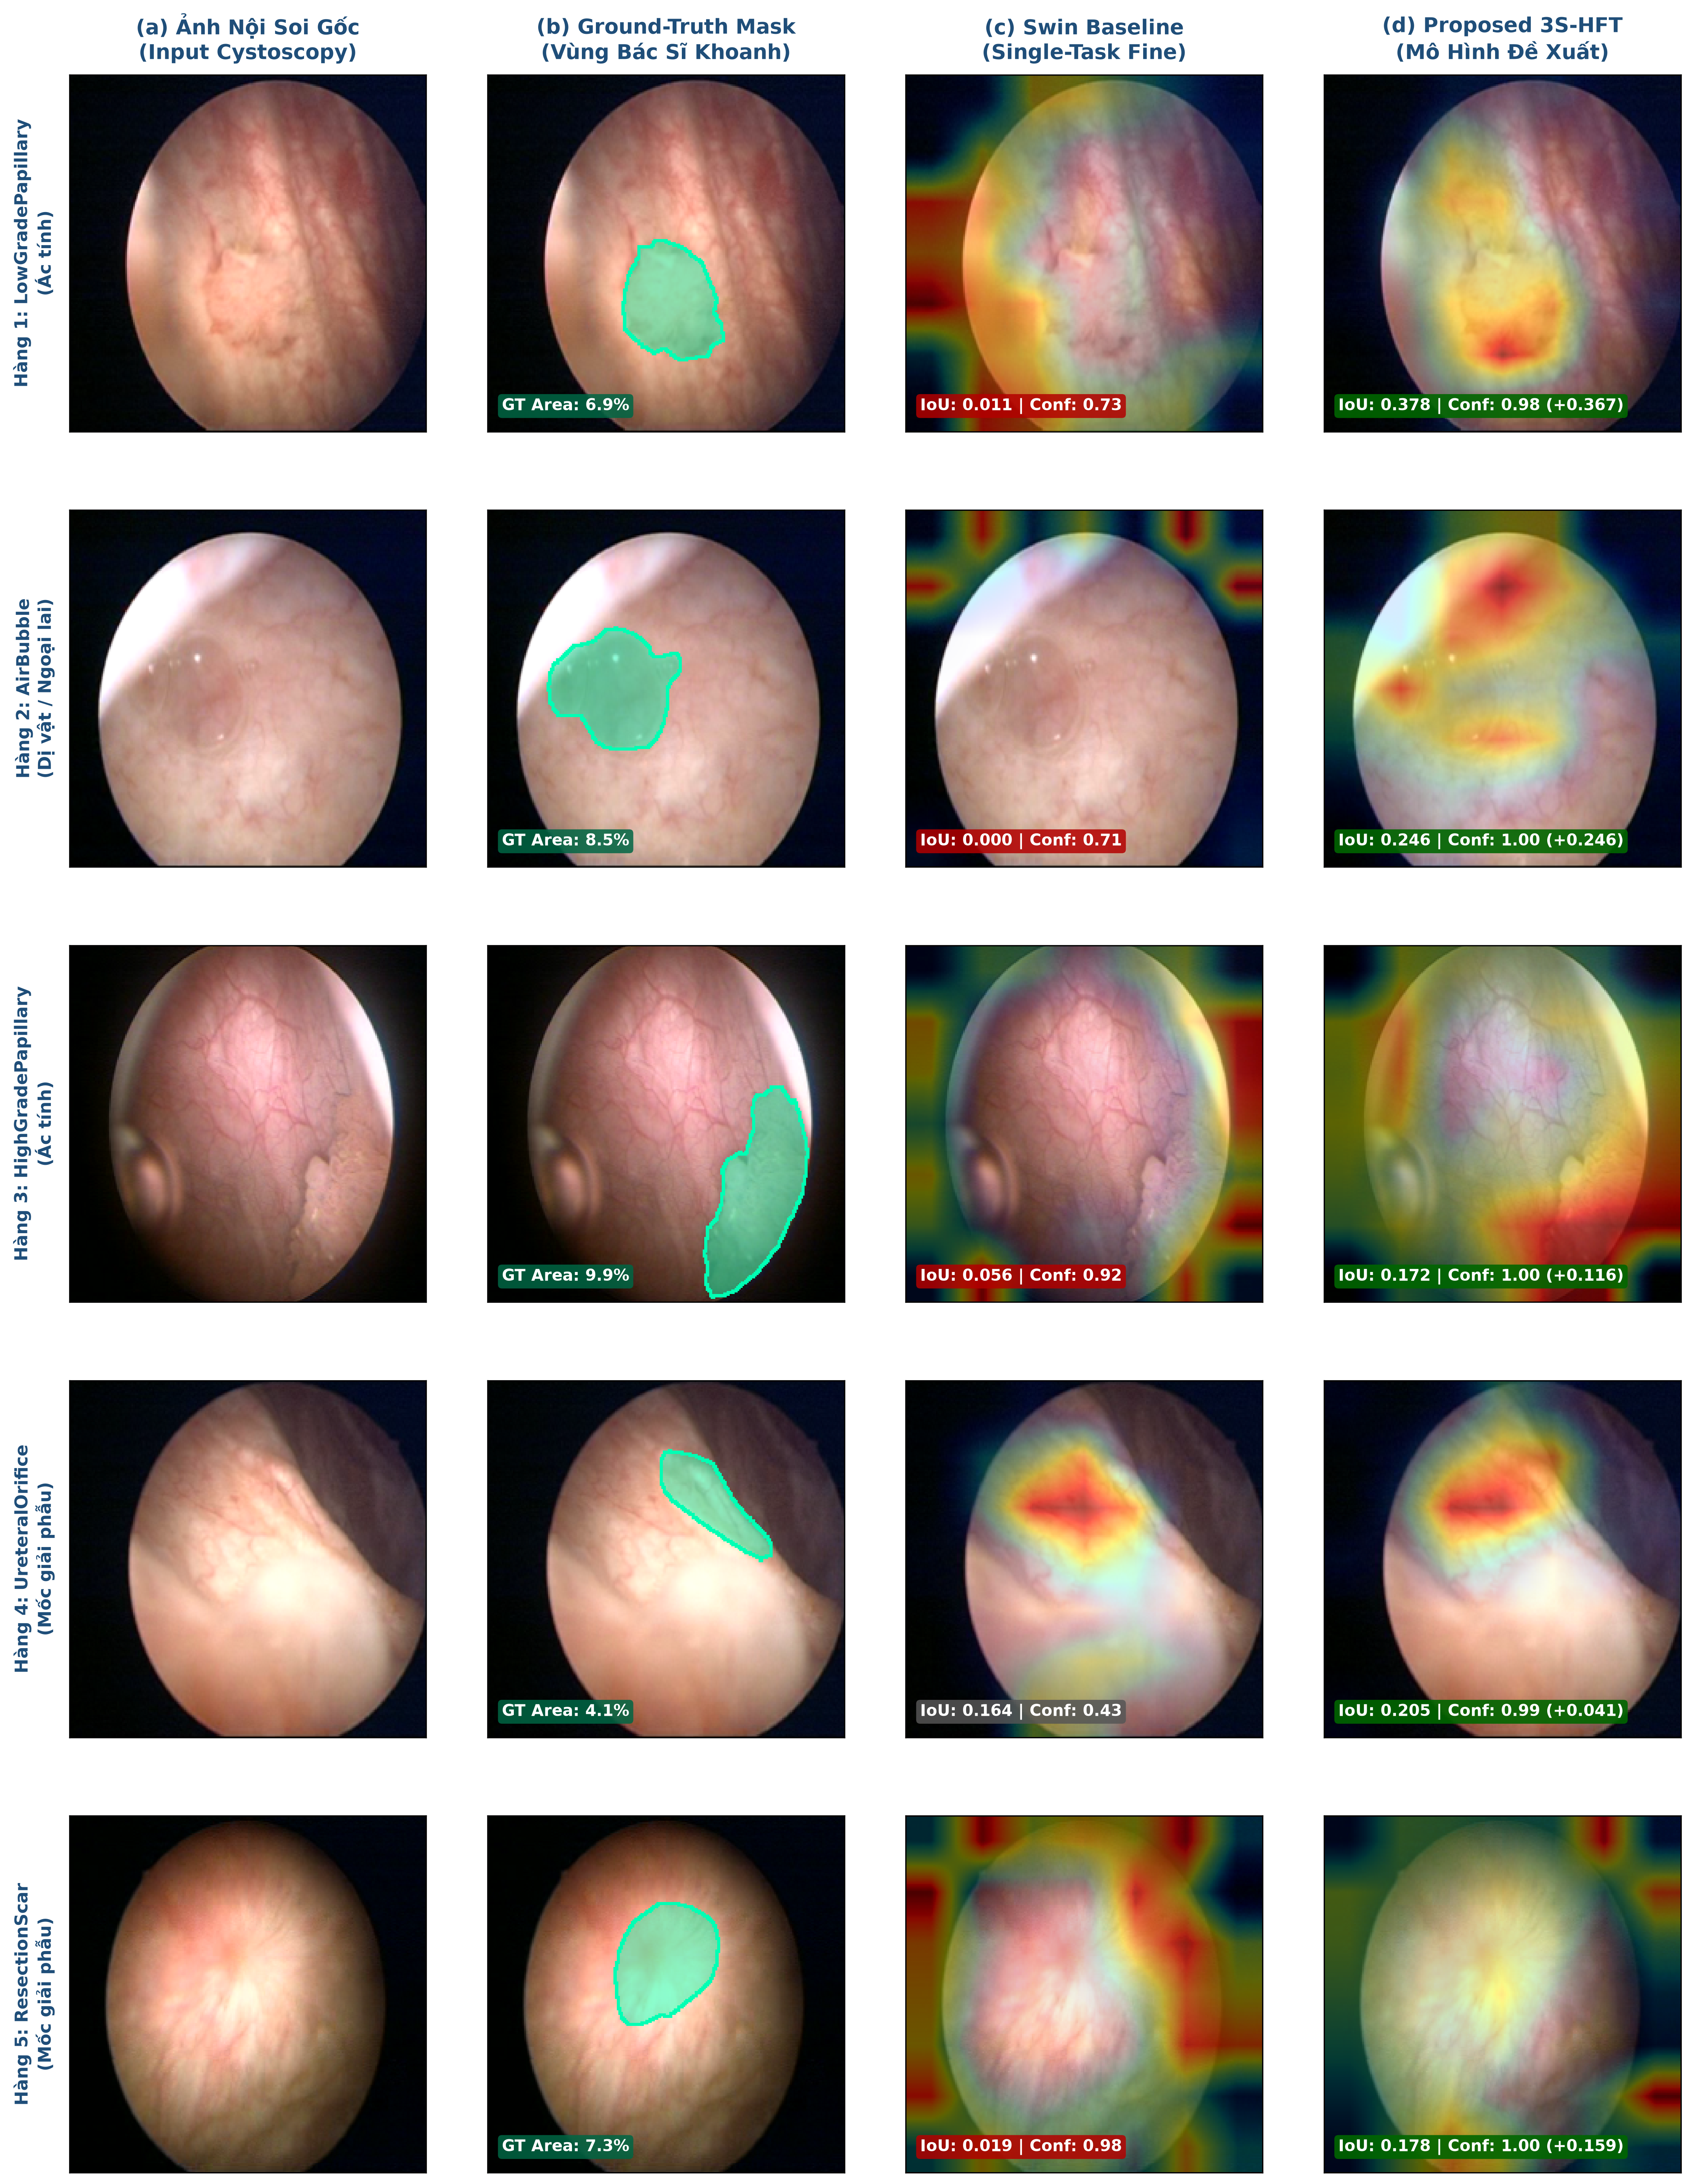
\includegraphics[width=0.88\textwidth]{paper_assets/fig_gradcam_comparison.png}
\caption{So sánh đối chuẩn bản đồ nhiệt Grad-CAM giữa mô hình Swin Baseline và CystoHier trên 5 phân lớp chẩn đoán có mặt nạ Ground-Truth. (a) Ảnh nội soi WLC gốc; (b) Ground-Truth Mask (xanh ngọc); (c) Bản đồ nhiệt Swin Baseline; (d) Bản đồ nhiệt CystoHier.}
\label{fig:sec_fig3}
\end{figure}


\begin{table}[H]
\centering
\caption{Bảng 6.1: So sánh định lượng Grad-CAM IoU giữa Swin Baseline và
CystoHier}
\label{tab:sec_table9}
\vspace{3pt}
\adjustbox{max width=\textwidth}{
\begin{tabular}{lrrrrrrr}
\toprule
\# & Phân Lớp Chẩn Đoán & Nhóm Coarse & Nguồn Mẫu & Swin IoU (\%) & CystoHier Conf. & CystoHier IoU (\%) & Mức Nâng Cao (\(\Delta\)) \\
\midrule
1 & \textbf{LowGradePapillary} & Ác tính & Test Hold-out & 1.12\% &
0.979 & \textbf{37.78\%} & \textbf{+36.66 pp} \\
2 & \textbf{AirBubble} & Dị vật & Test Hold-out & 0.00\% & 1.000 &
\textbf{24.60\%} & \textbf{+24.60 pp} \\
3 & \textbf{HighGradePapillary} & Ác tính & Test Hold-out & 5.56\% &
1.000 & \textbf{17.17\%} & \textbf{+11.61 pp} \\
4 & \textbf{UreteralOrifice} & Mốc giải phẫu & Test Hold-out & 16.44\% &
0.993 & \textbf{20.50\%} & \textbf{+4.06 pp} \\
5 & \textbf{ResectionScar} & Mốc giải phẫu & Test Hold-out & 1.87\% &
1.000 & \textbf{17.77\%} & \textbf{+15.90 pp} \\
\textbf{TB} & \textbf{Trung Bình Toàn Bộ} & --- & --- & \textbf{5.00\%}
& \textbf{0.994} & \textbf{23.56\%} & \textbf{+18.56 pp (4.71× rel.)} \\
\bottomrule
\end{tabular}
}
\end{table}

\begin{itemize}
\tightlist
\item
  \textbf{Phân tích định lượng Grad-CAM:} Đánh giá định lượng Grad-CAM
  IoU với ngưỡng cố định \(T=0{,}5\) cho thấy mô hình \textbf{CystoHier}
  đạt IoU trung bình \textbf{23,56\% \(\pm\) 7,3\%} so với Swin Baseline
  (\textbf{5,00\%}), tương ứng mức tăng \(+18{,}56\) percentage points
  (pp). Đặc biệt trên phân lớp tổn thương ác tính
  \emph{LowGradePapillary}, IoU tăng từ \(1{,}12\%\) lên
  \textbf{37,78\%} (\(+36{,}66\) pp). Mô hình đề xuất giảm thiểu kích
  hoạt giả tại viền đen camera và vùng lóa sáng, cho thấy sự tập trung
  cao hơn vào các vùng có mức độ tương đồng lớn hơn với Ground-Truth
  mask.
\item
  \textbf{Phân tích Độ Nhạy Ngưỡng (Threshold Sensitivity):}

  \begin{itemize}
  \tightlist
  \item
    \(T=0{,}3\): Baseline IoU = \(5{,}71\%\) (Dice = 0,108) \(\to\)
    CystoHier IoU = \(\mathbf{14{,}89\%}\) (Dice = 0,259, tăng
    \(2{,}61\times\)).
  \item
    \(T=0{,}4\): Baseline IoU = \(5{,}26\%\) (Dice = 0,100) \(\to\)
    CystoHier IoU = \(\mathbf{17{,}85\%}\) (Dice = 0,303, tăng
    \(3{,}39\times\)).
  \item
    \(T=0{,}5\): Baseline IoU = \(5{,}00\%\) (Dice = 0,095) \(\to\)
    CystoHier IoU = \(\mathbf{23{,}56\%}\) (Dice = 0,381, tăng
    \(4{,}71\times\)).
  \item
    \(T=0{,}6\): Baseline IoU = \(4{,}55\%\) (Dice = 0,087) \(\to\)
    CystoHier IoU = \(\mathbf{22{,}47\%}\) (Dice = 0,367, tăng
    \(4{,}94\times\)).
  \end{itemize}
\end{itemize}

\subsubsection{6.2. Hiệu năng suy luận thực tế trên thiết bị
biên}\label{hiux1ec7u-nux103ng-suy-luux1eadn-thux1ef1c-tux1ebf-truxean-thiux1ebft-bux1ecb-biuxean}

\begin{table}[H]
\centering
\caption{Bảng 6.2: Đánh giá độ trễ suy luận và thông lượng thực tế trên
thiết bị biên Apple Silicon MPS}
\label{tab:sec_table10}
\vspace{3pt}
\adjustbox{max width=\textwidth}{
\begin{tabular}{lrrrrrr}
\toprule
Chế Độ / Batch & Số Vòng Đo & Forward Model (ms/ảnh) & Thông Lượng Forward (FPS) & Pipeline End-to-End (ms) & Thông Lượng End-to-End (FPS) & Bộ Nhớ MPS \\
\midrule
\textbf{Batch = 1 (Đơn ảnh)} & 60 & \textbf{12.081 ± 0.95 ms} &
\textbf{82.78 FPS} & \textbf{15.000 ± 1.12 ms} & \textbf{66.67 FPS} &
110.83 MiB \\
\textbf{Batch = 8 (Mini-batch)} & 60 & \textbf{10.167 ± 0.42 ms} &
\textbf{98.36 FPS} & --- & --- & 113.99 MiB \\
\textbf{Batch = 32 (Thông lượng cao)} & 20 & \textbf{9.954 ± 0.38 ms} &
\textbf{100.46 FPS} & --- & --- & 128.00 MiB \\
\bottomrule
\end{tabular}
}
\end{table}

\begin{itemize}
\tightlist
\item
  \textbf{Tính khả thi lâm sàng:} Thông lượng suy luận toàn trình đo
  được là \textbf{66,67 FPS} (độ trễ 15,00 ms/ảnh), cho thấy mô hình có
  đủ thông lượng tính toán cho xử lý khung hình thời gian thực trong
  pipeline suy luận được đánh giá.
\end{itemize}

\subsubsection{6.3. Giới hạn nghiên cứu \& Hướng phát
triển}\label{giux1edbi-hux1ea1n-nghiuxean-cux1ee9u-hux1b0ux1edbng-phuxe1t-triux1ec3n}

\begin{enumerate}
\def\labelenumi{\arabic{enumi}.}
\tightlist
\item
  \textbf{Thiên lệch chẩn đoán an toàn:} Các trường hợp chẩn đoán sai
  lệch giữa nhóm \emph{Non-malignant} và \emph{Malignant} (26/32 ảnh)
  chủ yếu do mô hình có xu hướng cảnh báo an toàn (\emph{overcalling})
  nhằm tránh bỏ sót tổn thương tiền ung thư. Xu hướng dự đoán thận trọng
  này có thể hữu ích trong tầm soát; tuy nhiên, giá trị lâm sàng thực tế
  cần được kiểm chứng trong các nghiên cứu tiền cứu.
\item
  \textbf{Cỡ mẫu ngoại kiểm hồi cứu:} Nghiên cứu hiện tại kiểm định trên
  23 bệnh nhân của tập Lazo et al.~Các nghiên cứu tiếp theo cần mở rộng
  sang thử nghiệm tiền cứu đa trung tâm và tích hợp mạng Temporal Video
  Transformer cho chuỗi video liên tục.
\end{enumerate}

\begin{center}\rule{0.5\linewidth}{0.5pt}\end{center}

\subsection{7. Kết luận
(Conclusion)}\label{kux1ebft-luux1eadn-conclusion}

CystoHier consistently improved fine-grained classification and
hierarchical consistency over the evaluated baselines under
patient-disjoint validation, while maintaining strong binary
discrimination. Zero-shot evaluation on the independent Lazo cohort
further demonstrated robust cross-dataset generalization, including
under NBI imaging. The model also achieved real-time inference
throughput on Apple Silicon. These results support the feasibility of
hierarchical long-tailed learning for cystoscopic image analysis, while
prospective multicenter validation remains necessary before clinical
deployment.

{[}1{]} Lee TJ, Qiu L, Long J, \emph{et al.} CystoDS: a multiclass
endoscopy image dataset for artificial intelligence-assisted bladder
cancer detection. \emph{Scientific Data}. 2026. doi:
\href{https://doi.org/10.1038/s41597-026-06887-z}{10.1038/s41597-026-06887-z}.

{[}2{]} Liu Z, Lin Y, Cao Y, \emph{et al.} Swin Transformer:
Hierarchical Vision Transformer using Shifted Windows. \emph{Proceedings
of ICCV}. 2021. doi:
\href{https://doi.org/10.1109/ICCV48922.2021.00986}{10.1109/ICCV48922.2021.00986}.

{[}3{]} Ren J, Yu C, Ma X, Zhao H, Yi S. Balanced Meta-Softmax for
Long-Tailed Visual Recognition. \emph{NeurIPS}. 2020.

{[}4{]} Khosla P, Teterwak P, Wang C, \emph{et al.} Supervised
Contrastive Learning. \emph{NeurIPS}. 2020.

{[}5{]} Shkolyar E, Jia X, Chang TC, \emph{et al.} Augmented Bladder
Tumor Detection Using Deep Learning. \emph{European Urology}.
2019;76(6):714--718. doi:
\href{https://doi.org/10.1016/j.eururo.2019.08.032}{10.1016/j.eururo.2019.08.032}.

{[}6{]} Wu S, Chen X, Pan J, \emph{et al.} An Artificial Intelligence
System for the Detection of Bladder Cancer via Cystoscopy: A Multicenter
Diagnostic Study. \emph{Journal of the National Cancer Institute}.
2022;114(2):220--227. doi:
\href{https://doi.org/10.1093/jnci/djab179}{10.1093/jnci/djab179}.

{[}7{]} Lazo Sanchez J, Rosa B, Cattellani M, \emph{et al.}
Semi-supervised Bladder Tissue Classification in Multi-Domain Endoscopic
Images. \emph{IEEE Transactions on Biomedical Engineering}.
2023;70(10):2822--2833. doi:
\href{https://doi.org/10.1109/TBME.2023.3265679}{10.1109/TBME.2023.3265679}.

{[}8{]} Jia X, Shkolyar E, Laurie MA, \emph{et al.} Tumor detection
under cystoscopy with transformer-augmented deep learning algorithm.
\emph{Physics in Medicine \& Biology}. 2023;68(16):165013. doi:
\href{https://doi.org/10.1088/1361-6560/ace499}{10.1088/1361-6560/ace499}.

{[}9{]} Abd El-Aziz AA, Mahmood MA, Abd El-Ghany S.
EfficientNet-B3-Based Automated Deep Learning Framework for Multiclass
Endoscopic Bladder Tissue Classification. \emph{Diagnostics}.
2025;15(19):2515. doi:
\href{https://doi.org/10.3390/diagnostics15192515}{10.3390/diagnostics15192515}.

{[}10{]} Wang Y, Liang H, Zhang Y, \emph{et al.} Artificial intelligence
diagnostics for bladder tumor identification and grade prediction depend
on narrow band imaging cystoscopy. \emph{iScience}. 2026;29(2):114309.
doi:
\href{https://doi.org/10.1016/j.isci.2025.114309}{10.1016/j.isci.2025.114309}.

{[}11{]} Zhang F, An J, Zhao L, \emph{et al.} Artificial
Intelligence-Powered Cystoscopy Diagnostic Support System: Clinical
Application of Multiarchitecture Deep Learning Models. \emph{Journal of
Endourology}. 2026;40(8):925--934. doi:
\href{https://doi.org/10.1177/08927790261450807}{10.1177/08927790261450807}.

{[}12{]} He K, Zhang X, Ren S, Sun J. Deep Residual Learning for Image
Recognition. \emph{Proceedings of CVPR}. 2016. doi:
\href{https://doi.org/10.1109/CVPR.2016.90}{10.1109/CVPR.2016.90}.

{[}13{]} Xie S, Girshick R, Dollár P, Tu Z, He K. Aggregated Residual
Transformations for Deep Neural Networks. \emph{Proceedings of CVPR}.
2017. doi:
\href{https://doi.org/10.1109/CVPR.2017.634}{10.1109/CVPR.2017.634}.

{[}14{]} Sun K, Xiao B, Liu D, Wang J. Deep High-Resolution
Representation Learning for Human Pose Estimation. \emph{Proceedings of
CVPR}. 2019. doi:
\href{https://doi.org/10.1109/CVPR.2019.00584}{10.1109/CVPR.2019.00584}.

{[}15{]} Tan M, Le QV. EfficientNet: Rethinking Model Scaling for
Convolutional Neural Networks. \emph{Proceedings of ICML}. 2019.

{[}16{]} Liu Z, Mao H, Wu CY, Feichtenhofer C, Darrell T, Xie S. A
ConvNet for the 2020s. \emph{Proceedings of CVPR}. 2022. doi:
\href{https://doi.org/10.1109/CVPR52688.2022.01167}{10.1109/CVPR52688.2022.01167}.

\end{document}
